%!TEX TS-program = xelatex
%!TEX encoding = UTF-8 Unicode
%!TEX root = 2022-GS-ARTICLE.tex
%----------------------------------------------------------------- LANGUAGES ---
\newcommand{\mylanguages}{italian} % in reverse order
%---------------------------------------------------------- TITLE & SUBTITLE ---
\newcommand{\mytitle}{Totalità sonora: il corpo dell'orchestra}
\newcommand{\mysubtitle}{Per ascoltare l'organismo sonoro orchestrale nel suo complesso e nei singoli dettagli}
%----------------------------------------------------------------- AUTHOR(s) ---
\newcommand{\authorone}{Giancarlo Bottalico}
\newcommand{\institutione}{Conservatorio di musica "N. Piccinni", Bari}
\newcommand{\emailone}{giancarlobottalico@gmail.com}
%-------------------------------------------------------------------------------
% \newcommand{\authortwo}{Wikio Orgopedio}
% \newcommand{\institutiontwo}{Conservatorio S. Cecilia di Roma}
% \newcommand{\emailtwo}{wikio @ orgopedio.com} % duplicate these 3 lines if more
%-------------------------------------------------------------- STYLE GS2020 ---
%!TEX TS-program = xelatex
%!TEX encoding = UTF-8 Unicode
%!TEX root = 2022-GS-ARTICLE.tex
%-------------------------------- PACKAGES AND OTHER DOCUMENT CONFIGURATIONS ---
\documentclass[
	a4paper,
	twocolumn,
	twoside,
	%openright
]{article}
\usepackage[
	top=20mm,
	bottom=25mm,
	textwidth=17.2cm,
	columnsep=0.8cm,
	bindingoffset=1cm,
	showframe
]{geometry}
\usepackage[T1]{fontenc}
\usepackage[\mylanguages]{babel}
\usepackage{csquotes}
%\usepackage{parskip}
\usepackage[style=authoryear-ibid,backend=biber]{biblatex}
\bibliography{includes/bibliography.bib}
\usepackage{dblfloatfix}
\usepackage{subfigure}
\usepackage[subfigure]{tocloft}
\advance\cftsecnumwidth 0.5em\relax
\advance\cftsubsecindent 0.5em\relax
\advance\cftsubsecnumwidth 0.5em\relax
\usepackage{graphicx}
\usepackage{wrapfig}
% \usepackage{epstopdf}
% \epstopdfsetup{update}
\usepackage[usenames]{color}
\usepackage{xcolor}
\usepackage{tikz}
\usetikzlibrary{shapes,
                through,
								calc,
								intersections,
								backgrounds,
                positioning}
\usepackage{tkz-euclide}
\usepackage{amssymb}
\usepackage[
  colorlinks=true,
  linkcolor=black,
	anchorcolor=black,
	citecolor=black,
	filecolor=black,
	menucolor=black,
	runcolor=black,
	urlcolor=black
	]{hyperref}
\usepackage{Alegreya}
\linespread{1.05}
\usepackage{
	fontspec,
	xltxtra,
	xunicode
	}
\usepackage{
	xfrac,
	unicode-math
	}

\defaultfontfeatures{Mapping=tex-text}
\setmonofont[
	Scale=MatchLowercase
	]{Andale Mono}
\setmathfont[
	Scale=MatchLowercase,
	Scale=1
	]{Libertinus Math}

\usepackage{microtype}

\usepackage[
	hang,
	small,
	labelfont=bf,
	up,
	textfont=it,
	up
	]{caption}
\usepackage{paralist} % For compact item lists
\usepackage{etoolbox} % Some tools: used for quote environment
\AtBeginEnvironment{quote}{\small}
\usepackage{titling} % Customizing the title section
\usepackage{booktabs} % Horizontal rules in tables
\usepackage{enumitem} % Customized lists
\setlist[itemize]{noitemsep} % Make itemize lists more compact
\usepackage{abstract} % Allows abstract customization
\renewcommand{\abstractnamefont}{\normalfont\bfseries} % Set the "Abstract" text to bold
\renewcommand{\abstracttextfont}{\normalfont\small\itshape} % Set the abstract itself to small italic text
\usepackage{titlesec} % Allows customization of titles
\renewcommand\thesection{\Roman{section}} % Roman numerals for the sections
\renewcommand\thesubsection{\Roman{subsection}} % roman numerals for subsections
\titleformat{\section}[block]{\Large}{\thesection.}{1em}{} % Change the look of the section titles
\titleformat{\subsection}[block]{\large}{\thesubsection.}{1em}{} % Change the look of the section titles
%------------------------------------------------------------- TITLE SECTION ---
\setlength{\droptitle}{-4\baselineskip} % Move the title up
\pretitle{\begin{center}\huge\bfseries} % Article title formatting
\posttitle{\end{center}} % Article title closing formatting
\title{\mytitle \\[0.1cm] \large{\emph{\mysubtitle}}} % Article title
\author{%
\textsc{\authorone}\\%
\normalsize \institutione \\ %
\normalsize \emailone %
% activate
% \and % duplicate these 4 lines if more
% \textsc{\authortwo} \\%
% \normalsize \institutiontwo \\ %
% \normalsize \emailtwo %
}
\date{} % Leave empty to omit a date

\usepackage{fancyhdr} % Headers and footers
\pagestyle{fancy} % All pages have headers and footers
\fancyhead{} % Blank out the default header
\fancyfoot{} % Blank out the default footer
\fancyhead[C]{\small Wikipedia • General Relativity} % Custom header text
\fancyfoot[RO]{\small \today~ • w: \input{includes/words.txt} • c: \input{includes/char.txt} • p:~\thepage} % Custom footer text
\fancyfoot[LE]{\small p:~\thepage~ • c: \input{includes/char.txt} • w: \input{includes/words.txt} • \today} % Custom footer text

%-------------------------------------------------------------------------------
%-------------------------------------------------------------------------------
%	LISTINGS
%-------------------------------------------------------------------------------
%-------------------------------------------------------------------------------
\usepackage{listings}
% lstlistings setup
\definecolor{gsbg}{rgb}{0.98,0.98,0.98}

\lstset{%
  aboveskip=10pt,
	belowskip=5pt,
  language=C++,
  numbers=none,%left,%none,
  tabsize=4,
  %frame=single,
  breaklines=true,
  numberstyle=\tiny\ttfamily,
  backgroundcolor=\color{gsbg},
  basicstyle=\footnotesize\ttfamily,
  %commentstyle=\slshape\color{mylstcmt}, %\itshape,
  %frameround=tttt,
  columns=flexible, %fixed,
  showstringspaces=false,
  emptylines=2,
  inputencoding=utf8,
  extendedchars=true,
  literate=	{á}{{\'a}}1
			{à}{{\`a}}1
			{ä}{{\"a}}1
			{â}{{\^a}}1
			{é}{{\'e}}1
			{è}{{\`e}}1
			{ë}{{\"e}}1
			{ê}{{\^e}}1
			{ï}{{\"i}}1
			{î}{{\^i}}1
			{ö}{{\"o}}1
			{ô}{{\^o}}1
			{è}{{\`e}}1
			{ù}{{\`u}}1
			{û}{{\^u}}1
			{ç}{{\c{c}}}1
			{Ç}{{\c{C}}}1,
  emph={component, declare, environment, import, library, process},
  emph={[2]ffunction, fconstant, fvariable},
  emph={[3]button, checkbox, vslider, hslider, nentry, vgroup, hgroup, tgroup, vbargraph, hbargraph, attach},
  %emphstyle=\color{yotxt}, %\underline, %\bfseries,
  %morecomment=[s][\color{mylstdoc}]{<mdoc>}{</mdoc>},
  rulecolor=\color{black}
}

\usepackage[framemethod=tikz]{mdframed} % Allows defining custom boxed/framed environments

%-------------------------------------------------------------------------------
%--------------------------------------------------- INFORMATION ENVIRONMENT ---
%-------------------------------------------------------------------------------

% Usage:
% \begin{info}[optional title, defaults to "Info:"]
% 	contents
% 	\end{info}

\mdfdefinestyle{info}{%
	topline=false, bottomline=false,
	leftline=false, rightline=false,
	nobreak,
	singleextra={%
		\fill[black](P-|O)circle[radius=0.4em];
		\node at(P-|O){\color{white}\scriptsize\bf i};
		\draw[very thick](P-|O)++(0,-0.8em)--(O);%--(O-|P);
	}
}

% Define a custom environment for information
\newenvironment{info}[1][Info:]{ % Set the default title to "Info:"
	\medskip
	\begin{mdframed}[style=info]
		\footnotesize\noindent{\textbf{#1}}
}{
	\end{mdframed}
}

%-------------------------------------------------------------------------------
%----------------------------------------------------- BIOGRAFIA ENVIRONMENT ---
%-------------------------------------------------------------------------------

% Usage:
% \begin{bio}[optional title, defaults to "Info:"]
% 	contents
% 	\end{bio}

\mdfdefinestyle{bio}{%
	topline=false, bottomline=false,
	leftline=false, rightline=false,
	nobreak,
	singleextra={%
		\fill[black](P-|O)circle[radius=0.4em];
		\node at(P-|O){\color{white}\scriptsize\bf b};
		\draw[very thick](P-|O)++(0,-0.8em)--(O);%--(O-|P);
	}
}

% Define a custom environment for information
\newenvironment{bio}[1][Biografia:]{ % Set the default title to "Info:"
	\medskip
	\begin{mdframed}[style=bio]
		\noindent{\textbf{#1}}
}{
	\end{mdframed}
}

%-------------------------------------------------------------------------------
%------------------------------------------------------- WARNING ENVIRONMENT ---
%-------------------------------------------------------------------------------

% Usage:
% \begin{warn}[optional title, defaults to "Warning:"]
%	Contents
% \end{warn}

\mdfdefinestyle{warning}{
	topline=false, bottomline=false,
	leftline=false, rightline=false,
	nobreak,
	singleextra={%
		\draw(P-|O)++(-0.5em,0)node(tmp1){};
		\draw(P-|O)++(0.5em,0)node(tmp2){};
		\fill[black,rotate around={45:(P-|O)}](tmp1)rectangle(tmp2);
		\node at(P-|O){\color{white}\scriptsize\bf !};
		\draw[very thick](P-|O)++(0,-1em)--(O);%--(O-|P);
	}
}

% Define a custom environment for warning text
\newenvironment{warn}[1][Warning:]{ % Set the default warning to "Warning:"
	\medskip
	\begin{mdframed}[style=warning]
		\noindent{\textbf{#1}}
}{
	\end{mdframed}
}

%-------------------------------------------------------------------- ABSTRACT -
\renewcommand{\maketitlehookd}{%
\begin{abstract}
\noindent\input{includes/abstract.txt}
\end{abstract}
}

%------------------------------------------------------------ BEGIN DOCUMENT ---
\begin{document}
\maketitle
\thispagestyle{empty}
%-------------------------------------------------------------------- ABSTRACT -
% The abstract is an external txt file inside the includes folder
%-------------------------------------------------------------------------------
\section*{Disposizione dei microfoni}
Per la ripresa dell'intera orchestra sono stati utilizzati principalmente 2 tipi di microfoni:
\begin{compactitem} 
\item Microfono cardioide di marca Schoeps in configurazione stereofonica ORTF
\item 10 microfoni omni direzionali di modello OM1 di marca Line Audio organizzati in coppie stereofoniche in configurazione AB
\end{compactitem}
I microfoni sono stati disposti nello spazio come descritto nella mappa della figura 1.

\begin{figure}[t]
	\centering
	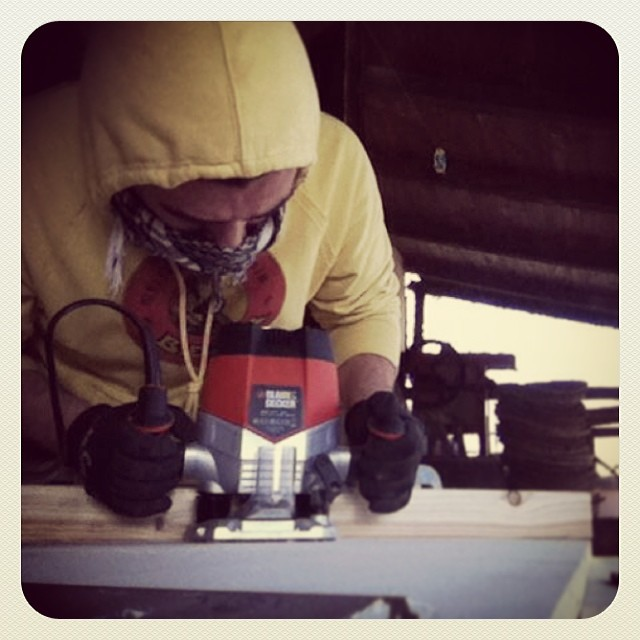
\includegraphics[width=.47\textwidth]{img/image2.jpg}
	\caption{Mappa della disposizione dei microfoni di Gabriele Acquafredda}
	\label{gs}
\end{figure}

\subsection*{Ruoli di ciascun punto di ripresa}
Ciascuno dei microfoni ha un ruolo preciso all'interno della ripresa dell'orchestra, in base a due parametri principali, ovvero:
\begin{compactitem}
\item Coppia stereofonica della quale è parte
\item Il suo posizionamento nello spazio: essendo i microfoni utilizzati identici tra loro (fatta eccezione per l'ORTF), il loro carattere dipende solo ed esclusivamente dal loro posizionamento.
\end{compactitem}
E' solo in base a questo che la sonorità dell'ambiente e della fonte sonora cambia nella ripresa.

\subsubsection*{L'ORTF}
Il punto di ripresa principale è costituito da un ORTF, ovvero una coppia stereofonica semi spaziata formata da due cardioidi posti ad una distanza di 17cm tra di loro (circa la stessa distanza che intercorre tra le orecchie in un cranio umano) inclinate di 110° circa.
La caratteristica principale del modello ORTF è la sua naturalezza: questa coppia semi-spaziata permette di riprendere l'ambiente in maniera tridimensionale, fornendo informazioni relative alla profondità dell'ambiente acustico. Permette di riprendere le fonti con i loro rispettivi ritardi, fornendo informazioni sulla reale provenienza del suono in base al ritardo che intercorre tra le due capsule microfoniche.
In questo caso, L'ORTF è stato posto di fronte all'orchestra in corrispondenza del pianoforte e del direttore, a fronte palco.

\subsubsection*{I 10 Line Audio modello OM1}
Osservando il diagramma polare e la risposta in frequenza del microfono omnidirezionale di marca Line Audio modello OM1 mostrato nella figura 2, si può evincere che questo microfono non è lineare in direzionalità: si comporta diversamente a seconda delle frequenze che cattura, ha la tendenza a limitare la sua direzionalità al crescere delle frequenze catturate stringendo la sua figura polare. Dal diagramma si può notare che il microfono è realmente omnidirezionale a 125 e a 2000 Hz, la sua digura polare si stringe di poco a 250 e a 4000 Hz. A 500 e a 8000, in particolar modo sul retro, la figura si stringe ancora sino ad essere attenuata di quasi 10dB a 1KHz e a 16KHz

\begin{figure}[b]
	\begin{center}
		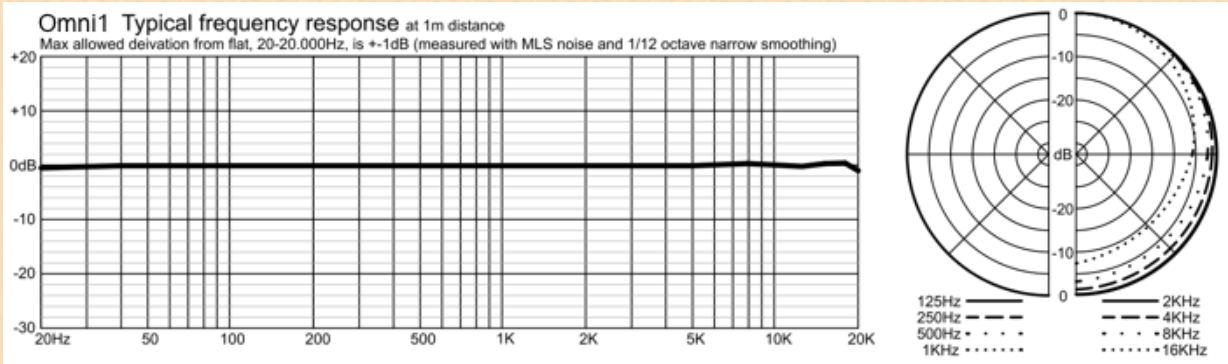
\includegraphics[width=.47\textwidth]{img/image1.png}
		\caption{\textbf{Caratteristiche del microfono di marca Line Audio modello Omni1}. Diagramma polare e risposta in frequenza.}
		\label{gr01}
	\end{center}
\end{figure}

I 10 microfoni sono stati organizzati in coppie stereofoniche AB, la quale prevede che essi siano distanziati ad una distanza variabile in base alle dimensioni della sorgente. In particolar modo:

\begin{enumerate}
\item Una coppia per i primi violini e per le viole, posizionati specularmente nell'orchestra a distanza di 425cm l'uno dall'altro.

\item Tre per i fiati, dei quali uno centrale e due laterali, per allargarne l'immagine. Per questa sezione sono stati utilizzati tre microfoni per due motivi principali:
\begin{compactitem}
	\item La sezione è molto ampia(428cm)
\item Per catturare anche i timpani, e in particolar modo il loro dettaglio, essendo storicamente utilizzati per dare sostegno ai fiati aggiungendo attacco e corpo al  suono.
\end{compactitem}

\item Una coppia a distanzata di 28cm per il pianoforte

\item Due utilizzati come Flanks, a distanza speculare di 324cm per allargare l'immagine stereo dell'ORTF. Il complesso Flanks + ORTF costituisce la ripresa MAIN dell'orchestra, ovvero quella generale, la quale non serve a catturare i singoli dettagli delle sezioni, quanto a dare un'immagine complessiva frontale del corpo dell'orchestra.

\item Uno come spot per i contrabbassi, posto a 309cm dal flankR. La sua utilità sta nel compensare il loro dettaglio che sicuramente manca al resto. C'è da precisare che questo punto di ripresa non potrebbe dare informazioni sulla profondità della sezione trattandosi di un microfono mono, così come non potrebbe riprenderne fedelmente le basse frequenze essendo un microfono di spot e quindi molto vicino alla sorgente.
\end{enumerate}

\section*{Gestione del materiale}
Premesso che:
\begin{compactitem}
\item Al fine di realizzare un complesso sonoro unitario, il posizionamento dei microfoni è stato pensato per riprendere i dettagli di ogni sezione
\item Il carattere timbrico di ogni singolo microfono dipende dalla sua posizione nello spazio
\end{compactitem}

Occorre organizzare le tracce affinchè ciascuna di esse abbia un ruolo preciso come componente del prodotto finale. Ma con quale criterio? Quale dominio di analisi restituisce l'immagine stereofonica più verosimile e solida? Le possibilità analizzate all'interno di questa ricerca sono due: dominio Left/Right e dominio Mid/Side

\subsection*{Dominio Left/Right}
Organizzare le tracce al fine di ascoltarle nel semplice dominio Left/Right vuol dire disporle longitudinalmente nell'immagine di ascolto senza alcuna informazione stereofonica relativa all'ambiente acustico nel quale suona l'orchestra o alla profondità della stessa.
Organizzare le tracce in questo modo equivale a creare un'immagine bidimensionale dell'orchestra: larghezza ed ampiezza, ma senza profondità.
É chiaro che le possibilità di analisi e di gestione del materiale sono limitate

\subsection*{Dominio Mid/Side}
Perchè analizzare il materiale delle registrazioni in Mid Side?
In questa configurazione, si può gestire l'ambiente come uno spazio trigonometrico, in quanto è possibile percepire la profondità di una fonte sonora nello spazio acustico nel quale suona, rimanendo fedeli al concetto di stereofonia.
Indagare il materiale in Mid/Side equivale a poter dominare una gestione tridimensionale dello spazio, e ovviamente le possibilità di analisi aumentano.
In fase d'ascolto, è utile mettere in correlazione le diverse coppie stereo con il punto di ripresa MAIN per potersi fare un'idea del posizionamento che  queste assumono nell'immagine stereo.

Una volta create le folder M/S per ciascuna coppia, equalizziamo separatamente Mid e Side facendo in modo che le frequenze gravi dominino nel Mid e viceversa, per evitare cancellazioni di fase tra i due e per orientare le bande dello spettro nella nostra immagine stereo, nella quale avremo il corpo, la presenza e le basse frequenze al centro, e le informazioni stereofoniche (relative quindi all'ambiente nel quale suona l'orchestra) sul Side. Così facendo avremo una configurazione nella quale è possibile percepire al contempo presenza, corpo, dettagli e informazioni relative allo spazio acustico.

\subsection*{Equalizzazione del materiale}
L'indagine del materiale in Mid/Side apre diversi vantaggi relativi alla gestione del materiale, come ad esempio sull'equalizzazione. Raggruppiamo le tracce in diverse folder tracks:
\begin{compactitem} 
	\item MAIN(ORTF, Flanks)
	\item FIATI(Fiati Left, Fiati Right, Fiati Center)
	\item VIOLINI/VIOLE(Secondi Violini, Viole).
	\item PIANOFORTE (Piano Left, Piano Right)
	\end{compactitem}
Con il fine di far emergere il dettaglio delle diverse sezioni dal timbro delle regitrazioni, le ho filtrate  in maniera non invasiva.
Ad esempio: Nelle registrazioni dei microfoni utilizzati per riprendere la sezione dei fiati ho attenuato le frequenze gravi, in quanto l'utilità di questo punto di ripresa è riprendere il dettaglio timbrico dei fiati e delle membrane dei timpani, i quali servono a sostenere i fiati. Le frequenze gravi dei timpani saranno già riprese fedelmente dai microfoni MAIN, trattandosi di microfoni lontani, dove la loro distanza dalla sorgente sonora permette a quest'ultima di svilupparsi per tutta la sua lunghezza d'onda.
Applico lo stesso ragionamento ai contrabbassi: attenuo le frequenze gravi dalle registrazioni del microfono utilizzato come spot, per mettere in risalto il suono timbrico della sezione dei contrabbassi.


\vfill\null

\newpage % USE NEWPAGE TO FORCE COLUMNN INTERRUPTION
%-------------------------------------------------------------------------------
%-------------------------------------------------------------------------------

\begin{table}[htp]
\begin{tabular}{ll}
\textbf{Sommario} & \textbf{Page} \\
\hline
\textbf{Disposizione dei microfoni} & 1 \\
Ruoli di ciascun punto di ripresa & \\
L'ORTF & \\
I 10 Line Audio modello Omni1 & \\
\hline
\textbf{Gestione del materiale} & 2 \\
Sessione di registrazione & \\
Trattamento del materiale Mid/Side & \\

\end{tabular}
\end{table}

%--------------------------------------------
%----------------larghezza massima del codice

\vfill\null

\raggedright
%\bibliographystyle{unsrt}
%\printbibliography

\end{document}

%%%%%%%%%%%%%%%%%%%%%%%%%%%%%%%%%%%%%%%%%%%%%%%%%%%%%%%%%%%%%%%%%%%%%%%%%%%%%%%%
% 2020 GIUSEPPE SILVI ARTICLE TEMPLATE BASED ON
%%%%%%%%%%%%%%%%%%%%%%%%%%%%%%%%%%%%%%%%%%%%%%%%%%%%%%%%%%%%%%%%%%%%%%%%%%%%%%%%
% Journal Article
% LaTeX Template
% Version 1.4 (15/5/16)
% This template has been downloaded from:
% http://www.LaTeXTemplates.com
% Original author:
% Frits Wenneker (http://www.howtotex.com) with extensive modifications by
% Vel (vel@LaTeXTemplates.com)
% License:
% CC BY-NC-SA 3.0 (http://creativecommons.org/licenses/by-nc-sa/3.0/)
%%%%%%%%%%%%%%%%%%%%%%%%%%%%%%%%%%%%%%%%%%%%%%%%%%%%%%%%%%%%%%%%%%%%%%%%%%%%%%%%
